\subsubsection{Seriel kommunikation}

\myparagraph{Devkit8000-PSoC Master}
\\
Som beskrevet i analysen for SPI (reference), blev denne protokol valgt pga. den kendskab gruppen allerede havde fra HAL øvelse 6 (reference). 
For at kunne kommunikere over SPI fra en Linux platform, skal den rette device driver indsættes i Linux kernen. Denne driver tillader os at tilgå
den SPI hardware som er på Devkittet fra vores grafiske brugergrænseflade. Ideen er at man skriver en driver der via det SPI interface som allerede er 
implemenret, kan lave metoder som gør det muligt at overfører data til/fra userspace(GUI).\\

I driveren skal opsætningen for SPI forbindelsen naturligvis også erklæret. Dette indebære bl.a. bus nummer, antal databits, maksimal overfølelses hastighed m.m.  
 
SPI device driveren fra øvelse 6 I HAL blev benyttet som udgangspunkt til at lave en tilpasset driver, som kunne kommunikere med PSoC Master. 
Denne forbindelse viste sig dog at volde store problemer for gruppen, og det lykkedes ikke at få hverken sendt eller modtaget data med denne driver.\\

Det blev herefter besluttes at der ikke skulle bruges mere tid på selv at lave en driver, og istedet benytte en SPI device driver som var udleveret fra skolen.
Dog var det blot den binære fil som var tilgængelig, hvilket betød at der ikke var adgang til source-koden. Dette gjorde at gruppen ikke kunne tilpasse driveren,
og alt information omkring opsætningen for SPI forbindelse måtte udledes fra det PSoC-Creator program som medfulgte. 

\begin{figure}[H]
	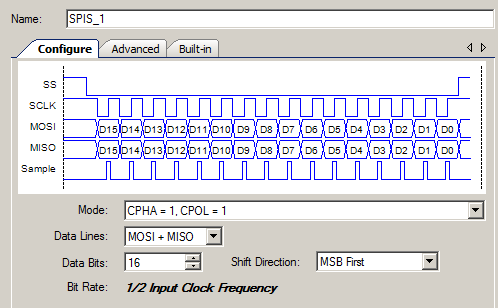
\includegraphics[scale=0.6]{tex/Design/SPI/Clock_mode_SPI}
	\caption{Opsætning for SPI forbindelse Devkit8000-PSoC Master}
	\label{SPI_opsaetning}
\end{figure}

Ud fra figur \ref{SPI_opsaetning}, kan det aflæses at SPI clock mode er sat til CPHA = 1 og CPOL = 1, og antal databits sat til 16. Det PSoC program som var udleveret blev brugt
som skabelon for gruppens eget program til PSoC master, dog med nogle modifikationer. Især håndteringen af de databits som blev modtaget fra devkittet blev 
genbrugt, da der ikke kunne ændres på disse bitkombinationer. For information omkring implementeringen af håndtering af databits for SPI kommunikation, 
henvises til afsnittet "Implementering".

\myparagraph{PSoC Master - PSoC Slave}
\\
Til SPI forbindelsen mellem PSoC Master og PSoc slave havde gruppen frie hænder til opsætte SPI. Her blev clock mode valgt til CHPA = 0 og CPOL = 0, og 
antal databits til 8. Grunden til der kun bliver sendt 8 bits her, er at det er tilstrækkeligt til den simple form for kommunikation der er mellem PSoc enhederne.
8 databits ville også have været fint for Devkit-PSoC forbindelsen, men som tidligere nævnt kunne det ikke ændres da der ikke var adgang til SPI device driveren
på Devkit8000. Clock mode er ændret til default værdien fra PSoC-Creator, hvilket der ikke har været nogen yderlige designmæssige tanker omkring.